\section{图同构}
\label{sec:graph-isomorphism}

顶点的名称只是为了区分顶点而取的。把贯穿图的顶点换一套编号，边集的写法会变，邻接矩阵的行列也会移动，连接结构本身却没有变。比较两张图时，需要一个标准来判断它们是否只差一套名称。本节先用保持邻接的一一对应定义同构，再用第~\ref{sec:prelim-common-matrices}小节的置换矩阵把重编号写成矩阵运算。怎样系统地比较两张图的结构，是第~\ref{sec:graph-wl-refinement}节的内容；这里先把要判定的目标说清楚。

\subsection{图同构的定义}
\label{sec:graph-conn-isomorphism-definition}

图~\ref{fig:graph-conn-isomorphism}(a)是贯穿图$\mathcal G$；(c)的$\mathcal G'$顶点集也是$\{1,2,3,4\}$，边集由$\{1,3\}$、$\{1,4\}$、$\{2,3\}$、$\{2,4\}$、$\{3,4\}$组成，画出来有两条边交叉，看上去与菱形不同。若按(b)的规则$\rho$把$\mathcal G$的顶点改名，$\mathcal G$的五条边依次变为
\[
\begin{gathered}
\{1,2\}\mapsto\{1,3\},\qquad
\{1,3\}\mapsto\{1,4\},\qquad
\{2,3\}\mapsto\{3,4\},\\
\{2,4\}\mapsto\{3,2\},\qquad
\{3,4\}\mapsto\{4,2\},
\end{gathered}
\]
恰好是$\mathcal G'$的全部边；唯一不相邻的一对$\{1,4\}$变为$\{1,2\}$，在$\mathcal G'$中也不相邻。两张图只差一套名称。

\begin{figure}[!htb]
  \centering
  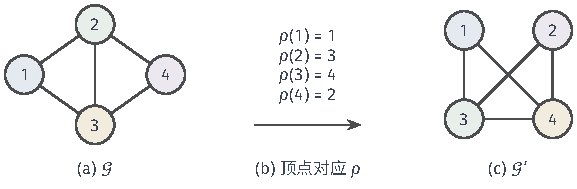
\includegraphics[width=97.688mm]{figures/01-basic-mathematics/04-graphs/tikz/c1-isomorphism-relabeling/figure.pdf}
  \caption{两张同构的图。(a)贯穿图$\mathcal G$；(c)画法与编号都不同的$\mathcal G'$；(b)顶点对应$\rho$。同色顶点互相对应：$\mathcal G$中顶点$i$与$\mathcal G'$中顶点$\rho(i)$颜色相同。逐条核对可见，$\mathcal G$中相邻的顶点对恰好对应$\mathcal G'$中相邻的顶点对。}
  \label{fig:graph-conn-isomorphism}
\end{figure}

\begin{definition}[图同构]
\label{def:graph-conn-isomorphism}
设$\mathcal G=(V,E)$与$\mathcal G'=(V',E')$是无向图。若存在双射$\rho:V\to V'$，使对任意$i,j\in V$都有
\[
\{i,j\}\in E\iff\{\rho(i),\rho(j)\}\in E',
\]
就称$\mathcal G$与$\mathcal G'$\term{同构}（isomorphic），称$\rho$为一个同构映射。
\end{definition}

定义中的双向条件不能减弱为单向。若只要求“$\mathcal G$的边映为$\mathcal G'$的边”，那么把边集为$\{1,2\},\{2,3\}$的路径按恒等映射放进三角形$\{1,2,3\}$也满足要求，但三角形多出了边$\{1,3\}$，两张图的边数不同。反方向的条件保证$\mathcal G'$中不出现$\mathcal G$里没有的连接，即保持不相邻关系。

\paragraph{有向图、加权图与带属性的图}
附加信息越多，同构要保持的东西越多。有向图的同构要求$(i,j)\in E\iff(\rho(i),\rho(j))\in E'$，即保持弧的方向；单向链$1\to2\to3$与$1\to2\leftarrow3$的底层无向图相同，作为有向图却不同构：后者的顶点$2$入度为$2$，前者每个顶点的入度至多为$1$，而有向图的同构映射保持入度。加权图还要求对应的边权相等，$w'_{\rho(i),\rho(j)}=w_{i,j}$；带属性的图则要由问题声明哪些属性必须保持，例如比较两个分子时原子种类必须一致，而原子的编号无关紧要。

\paragraph{用不变量排除同构}
同构映射保持一切由连接结构定义的量：顶点数、边数、每个顶点的度（$\rho$把$i$的邻居一一映为$\rho(i)$的邻居），因而还有全部顶点的度构成的多重集合，以及连通分量的个数、三角形的个数等。这些量称为图的不变量。只要有一个不变量不同，两张图就不同构。例如六个顶点排成一个环，与两个互不相连的三角形相比，顶点数、边数都是$6$，每个顶点的度都是$2$，但前者连通、后者有两个分量，所以不同构。

不变量相同却不足以断定同构。考虑两棵六个顶点的树，边集分别为
\[
\bigl\{\{1,2\},\{1,3\},\{1,4\},\{2,5\},\{3,6\}\bigr\}
\quad\text{与}\quad
\bigl\{\{1,2\},\{1,3\},\{1,4\},\{2,5\},\{5,6\}\bigr\}.
\]
二者都连通、没有三角形，度的多重集合都是$\{3,2,2,1,1,1\}$。但在前一棵树中，唯一的度为$3$的顶点$1$与两个度为$2$的顶点$2,3$相邻；在后一棵树中，顶点$1$只与一个度为$2$的顶点$2$相邻，另一个度为$2$的顶点$5$不是它的邻居。同构映射必须把度为$3$的顶点映到度为$3$的顶点，并保持它的邻居及邻居的度，所以两棵树不同构。这个例子提示，比较“邻居的度”能区分只看度区分不了的图；第~\ref{sec:graph-wl-refinement}节的顶点标记细化正是把这一想法反复执行。逐个尝试全部$n!$个双射虽然总能判定，但随$n$增长得太快，不能作为实用的方法。

\subsection{重编号与置换表示}
\label{sec:graph-conn-relabeling}

当两张图的顶点集都是$\{1,\ldots,n\}$时，同构映射$\rho$就是一个重编号：把顶点$i$改称为$\rho(i)$。重编号以后，邻接矩阵的行和列都要按同样的方式重新排列。第三部分的置换矩阵恰好执行这种重排。

\paragraph{置换共轭}
按第~\ref{sec:prelim-common-matrices}小节，取置换矩阵$\bm P=\begin{bmatrix}\bm e_{\rho(1)}&\cdots&\bm e_{\rho(n)}\end{bmatrix}$，它满足$\bm P\bm e_i=\bm e_{\rho(i)}$。由第~\ref{sec:ls-matrix-operations}小节置换矩阵的乘法规则，左乘$\bm P$把第$i$行移到第$\rho(i)$行；右乘$\bm P^{\top}$相当于对转置后的矩阵左乘$\bm P$，把第$j$列移到第$\rho(j)$列。两者合起来，
\begin{equation}
\bm A'=\bm P\bm A\bm P^{\top},\qquad
a'_{\rho(i),\rho(j)}=a_{i,j}.
\label{eq:graph-conn-relabel}
\end{equation}
第二式说明，原来记录“$i,j$是否相邻”的条目被搬到了新编号$\rho(i),\rho(j)$的位置。因此，$\rho$是$\mathcal G$到$\mathcal G'$的同构映射，当且仅当$\mathcal G'$的邻接矩阵等于$\bm P\bm A\bm P^{\top}$。

\paragraph{核对贯穿图的例子}
对图~\ref{fig:graph-conn-isomorphism}的$\rho$，$\bm P$的各列依次为$\bm e_1,\bm e_3,\bm e_4,\bm e_2$。由式\eqref{eq:graph-conn-running-adjacency}计算得
\[
\bm P=
\begin{bmatrix}
1&0&0&0\\
0&0&0&1\\
0&1&0&0\\
0&0&1&0
\end{bmatrix},\qquad
\bm P\bm A\bm P^{\top}=
\begin{bmatrix}
0&0&1&1\\
0&0&1&1\\
1&1&0&1\\
1&1&1&0
\end{bmatrix}.
\]
右边矩阵的第$1$行在第$3,4$列为$1$，即$N'(1)=\{3,4\}$；第$4$行在第$1,2,3$列为$1$，即$N'(4)=\{1,2,3\}$；各行都与$\mathcal G'$的边集一致。逐个位置看也是如此，例如$a'_{3,2}=a'_{\rho(2),\rho(4)}=a_{2,4}=1$。加权图把$\bm A$换成$\bm W$，同样要求$\bm W'=\bm P\bm W\bm P^{\top}$；允许零权边时，还要同时检验结构掩码$\bm M'=\bm P\bm M\bm P^{\top}$，因为两个顶点之间无边与有一条零权边，权矩阵都是零矩阵。

\paragraph{置换不同于一般换基}
置换矩阵满足$\bm P^{\top}\bm P=\bm I$，所以$\bm P^{\top}=\bm P^{-1}$，式\eqref{eq:graph-conn-relabel}是第~\ref{sec:ls-similarity}小节意义下的相似变换。但反过来，一般的相似变换$\bm S\bm A\bm S^{-1}$不能都解释为重编号。例如对两个顶点一条边的图，$\bm A=\left[\begin{smallmatrix}0&1\\1&0\end{smallmatrix}\right]$，取$\bm S=\left[\begin{smallmatrix}1&1\\0&1\end{smallmatrix}\right]$，得到
\[
\bm S\bm A\bm S^{-1}
=\begin{bmatrix}1&1\\0&1\end{bmatrix}
\begin{bmatrix}0&1\\1&0\end{bmatrix}
\begin{bmatrix}1&-1\\0&1\end{bmatrix}
=\begin{bmatrix}1&0\\1&-1\end{bmatrix},
\]
它不对称，有非零对角元和负条目，已经不是任何简单无向图的邻接矩阵。一般换基会把不同顶点的坐标混合起来，而重编号只搬动位置、不混合数值。相似变换保持特征值，所以同构的图有相同的邻接矩阵特征值；这一事实的用途和局限在第~\ref{chap:graph-spectral}章讨论，这里只确定重编号的精确含义。
